 % -*- root: ../../twm.tex -*-

 \section{Topic Modeling}

\begin{frame}
    \frametitle{Topic Modeling}
\begin{itemize}
    \item Group similar documents
    \item Dimension reduction for documents
\end{itemize}
\begin{itemize}
    \item Latent Semantic Analysis (LSA)
    \begin{itemize}
    \item Singular value decomposition (SVD)
    \end{itemize}
    \end{itemize}
\begin{itemize}
    \item {\color{iseblue}Blei et al (2003)}: Latent Dirichlet Allocation (LDA)
    \begin{itemize}
    \item Generative statistical model
    \item Document as mixture of topics
    \end{itemize}
\end{itemize}

\end{frame}

 \begin{frame}
    \frametitle{Top Terms in Topics}
\begin{center}
\begin{tabular}{ c | c c c c }
\hline
\hline
Topic & t1 & t2 & t3 & t4 \\
\hline
1 & light & malt & nice & s \\
2 & lager & butter & beer & taste \\
3 & chocolate & coffee & dark & porter  \\
4 & -pron- & beer & pumpkin & brew \\
5 & hop & light & malt & citrus  \\
 \hline
 \hline
\end{tabular}
\end{center}

\begin{itemize}
    \item Topic 2: light beers
    \item Topic 3: dark beers
\end{itemize}
\end{frame}

 \begin{frame}
    \frametitle{Top Topic}
\begin{figure}[htb]
\centering
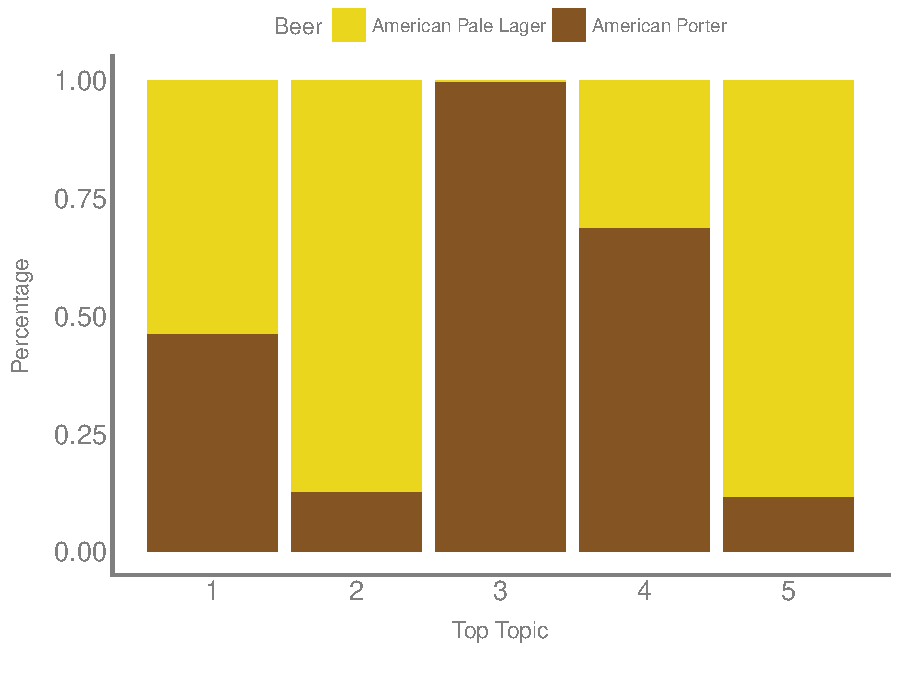
\includegraphics[scale=0.6]{img/figures/topic_stacked_1gram}
\end{figure}
\end{frame}

 \begin{frame}
    \frametitle{Topic Values}
\begin{figure}[htb]
\centering
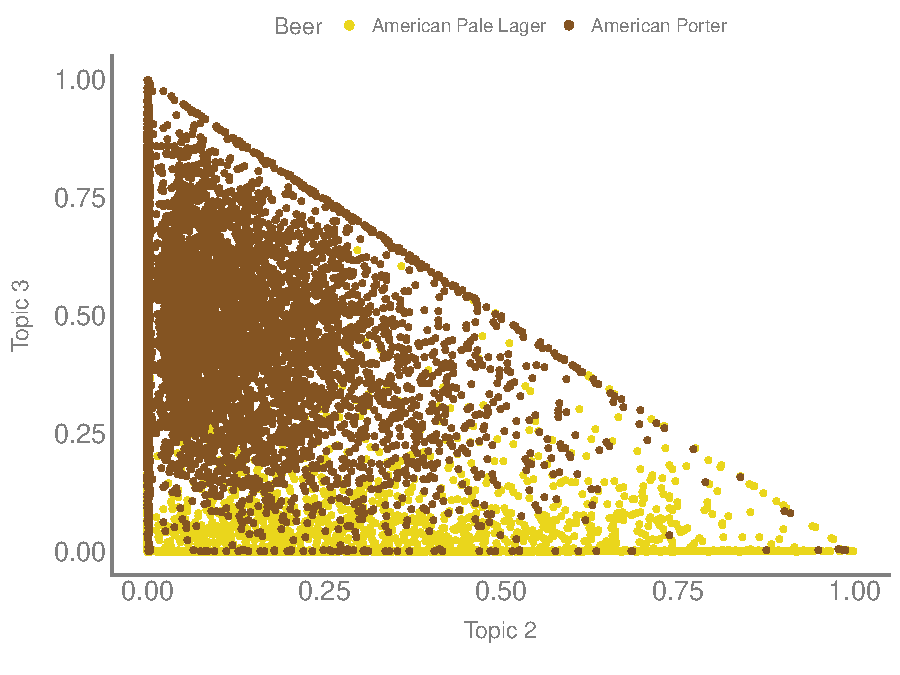
\includegraphics[scale=0.6]{img/figures/topic_scatter_1gram}
\end{figure}
\end{frame}

 \begin{frame}
    \frametitle{Discrimination Possible?}
\begin{itemize}
    \item Classify style by topic value
    \item Discrimination rule
\end{itemize}

\vspace{-5pt}
\begin{center}
{\color{iseblue}
    Lager if Topic 2 > Topic 3
}
\end{center}

\vspace{10pt}

{
\renewcommand{\arraystretch}{1.5}
\setlength{\tabcolsep}{.8em}
\begin{lvbtab}{ht}
\centering
\begin{tabular}{l|S[table-format=5.0]S[table-format=5.0]}
  \hline
\hline
\multicolumn{1}{c|}{\diagbox[width=5.5em]{True}{Pred}} &
\multicolumn{1}{c}{Porter}   &
\multicolumn{1}{c}{Lager}  \\ 
  \hline
Porter & 10559 & 616 \\ 
Lager & 859 & 5991 \\ 
\hline
\hline
\end{tabular}
\end{lvbtab}
}

\end{frame}


 \begin{frame}
    \frametitle{Top Terms in Topics - 2-grams}
\begin{center}
\begin{tabular}{ c | c c c c }
\hline
\hline
Topic & t1 & t2 & t3 \\
\hline
1 & tan head & dark fruit & dark brown \\
2 & dark chocolate & roasted malt & peanut butter \\
3 & white head & light body & pale lager  \\
4 & white head & floral hop & earthy hop \\
5 & pint glass & good beer & half  \\
 \hline
 \hline
\end{tabular}
\end{center}

\begin{itemize}
    \item Topic 1: dark beers
    \item Topic 3: light beers
    \item Topic 2, 4: taste and color
    \item Topic 5: general
\end{itemize}
\end{frame}

 \begin{frame}
    \frametitle{Top Topic - 2-grams}
\begin{figure}[htb]
\centering
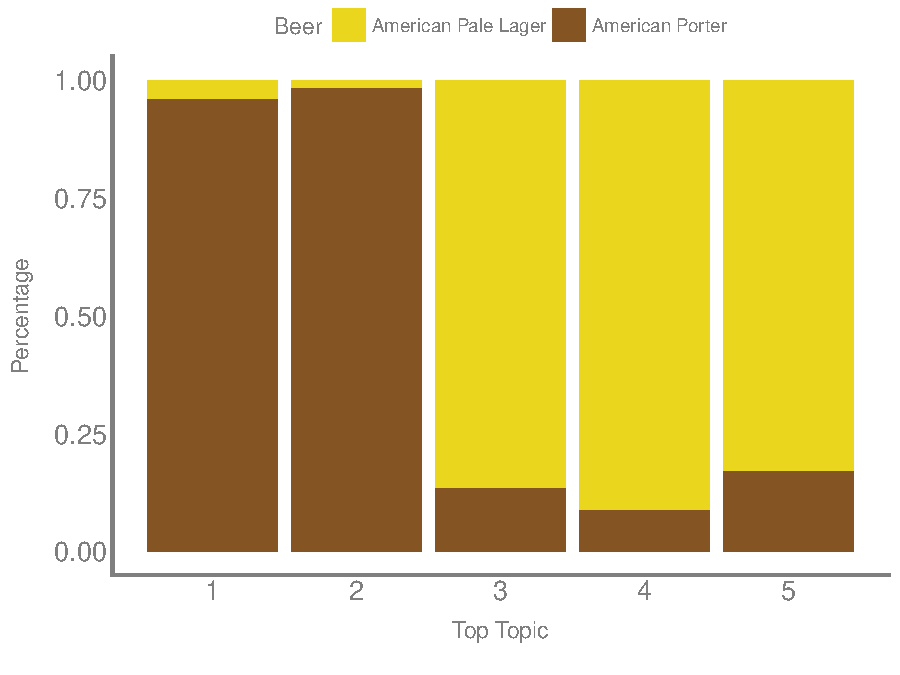
\includegraphics[scale=0.6]{img/figures/topic_stacked}
\end{figure}
\end{frame}

 \begin{frame}
    \frametitle{Topic Values - 2-grams}
\begin{figure}[htb]
\centering
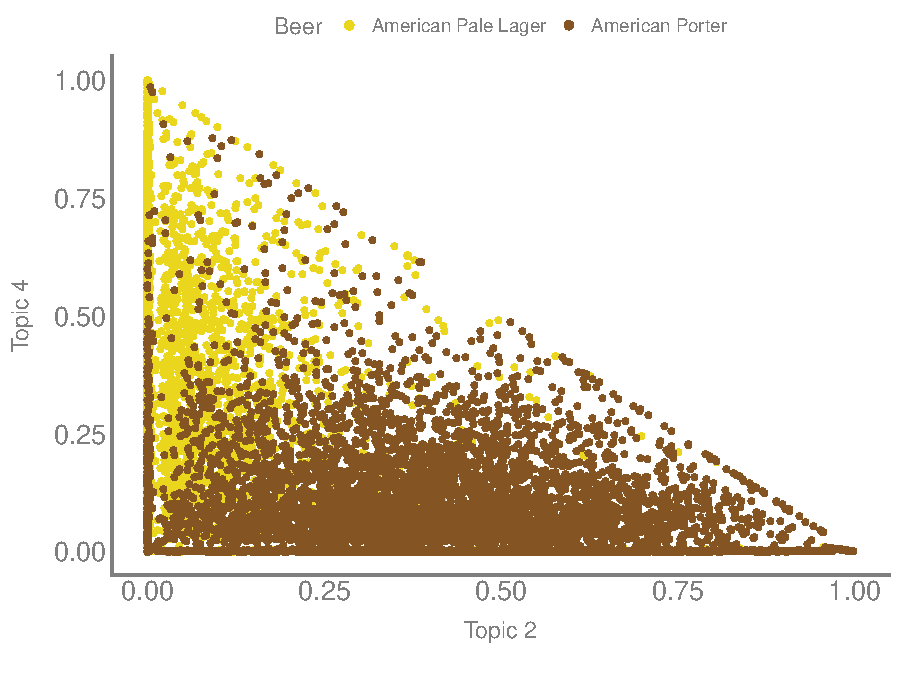
\includegraphics[scale=0.6]{img/figures/topic_scatter}
\end{figure}
\end{frame}

 \begin{frame}
    \frametitle{Topic Values - 2-grams ctd}
\begin{figure}[htb]
\centering
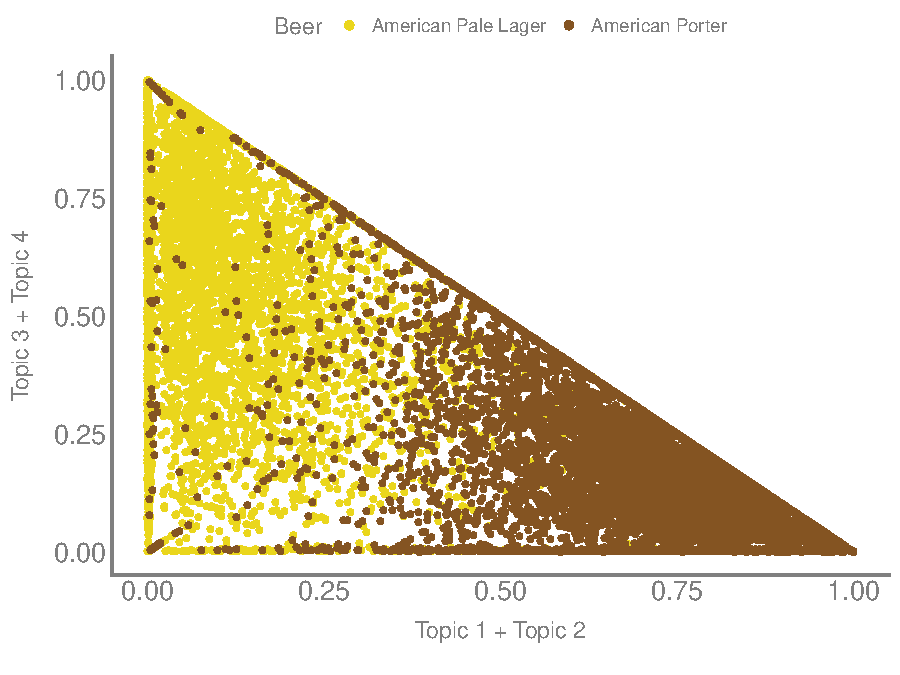
\includegraphics[scale=0.6]{img/figures/topic_scatter_additive}
\end{figure}
\end{frame}

 \begin{frame}
    \frametitle{Discrimination Possible? 2-grams}
\begin{itemize}
    \item Classify style by topic value
    \item Discrimination rule
\end{itemize}
\vspace{-10pt}
\begin{center}
{\color{iseblue}
    Lager if Topic 3 + Topic 4 > Topic 2 + Topic 1
}
\end{center}

\vspace{10pt}

{
\renewcommand{\arraystretch}{1.5}
\setlength{\tabcolsep}{.8em}
\begin{lvbtab}{ht}
\centering
\begin{tabular}{l|S[table-format=5.0]S[table-format=5.0]}
  \hline
\hline
\multicolumn{1}{c|}{\diagbox[width=5.5em]{True}{Pred}} &
\multicolumn{1}{c}{Lager}   &
\multicolumn{1}{c}{Porter}  \\ 
  \hline
Lager &  10723 &  452 \\ 
Porter & 616 & 6234 \\ 
\hline
\hline
\end{tabular}
\end{lvbtab}
}

\end{frame}

 \begin{frame}
    \frametitle{Drawbacks of LDA}
\begin{itemize}
    \item Fixed number of topics
    \item Non-hierarchical
    \item Static
    \item Number of documents and length is crucial
\end{itemize}
\end{frame}